%This is part of Un soupçon de mathématique sans être agressif pour autant
% Copyright (c) 2012-2014
%   Laurent Claessens
% See the file fdl-1.3.txt for copying conditions.

%+++++++++++++++++++++++++++++++++++++++++++++++++++++++++++++++++++++++++++++++++++++++++++++++++++++++++++++++++++++++++++ 
\section{Objectifs du chapitre}
%+++++++++++++++++++++++++++++++++++++++++++++++++++++++++++++++++++++++++++++++++++++++++++++++++++++++++++++++++++++++++++

Le but de ce chapitre est de voir la notion de fonction affine.
\begin{enumerate}
    \item
        La forme \( x\mapsto mx+p\).
    \item
        Un peu de lecture graphique : parler d'image et d'antécédents.
    \item
        Représentation graphique : signe de \( m\), coefficient directeur et ordonnée à l'origine.
    \item
        Tableau de signe.
    \item
        Résolution des équations correspondantes.
\end{enumerate}
Nous ne parlerons pas d'équation de droite à proprement parler. Donc pas de graphes de fonctions passant par deux points donné.

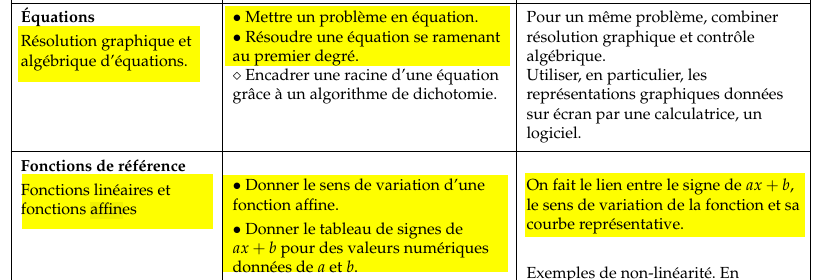
\includegraphics[width=\linewidth]{BO_fonctions_affines1}

\vspace{1cm}

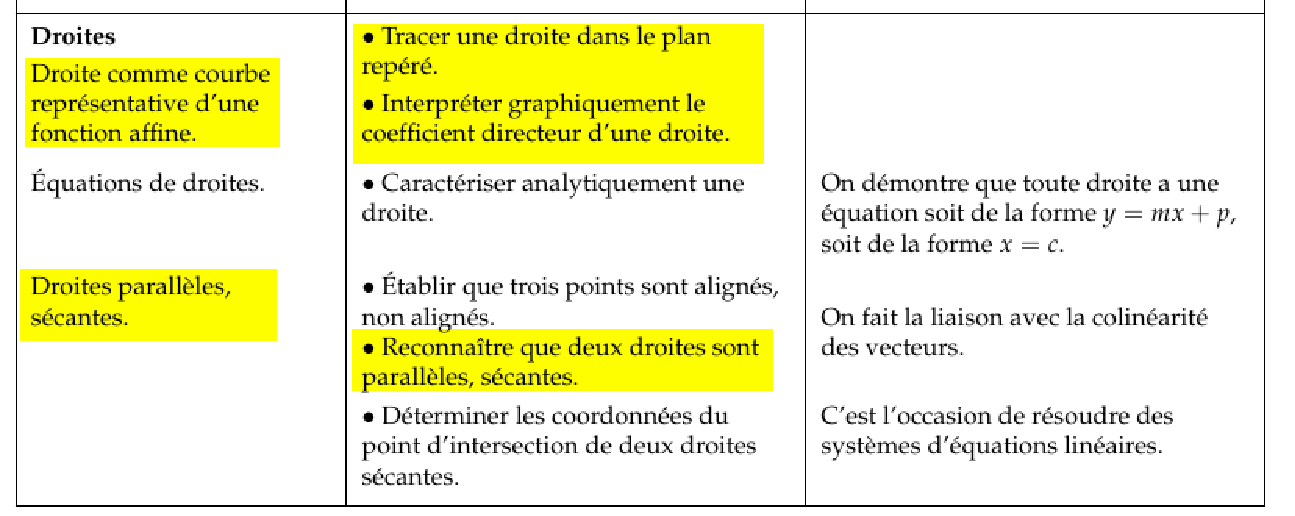
\includegraphics[width=\linewidth]{BO_fonctions_affines2}

%+++++++++++++++++++++++++++++++++++++++++++++++++++++++++++++++++++++++++++++++++++++++++++++++++++++++++++++++++++++++++++ 
\section{L'activité}
%+++++++++++++++++++++++++++++++++++++++++++++++++++++++++++++++++++++++++++++++++++++++++++++++++++++++++++++++++++++++++++

%This is part of Un soupçon de mathématique sans être agressif pour autant
% Copyright (c) 2012-2013
%   Laurent Claessens
% See the file fdl-1.3.txt for copying conditions.

    Le taxi Besacdanslesac divise son prix en deux parties : $0.2$ euros de frais de prise en charge plus un euro par km parcouru. Le taxi Ledoubstoudoux par contre divise son prix en $1$ euro de frais de prise en charge plus $0.8$ euros par kilomètre parcouru.

    \begin{enumerate}
        \item
            Combien coûte un trajet de \SI{5}{\kilo\meter} avec Besacdanslesac ?
        \item
            Donner une expression algébrique du prix d'une course en fonction du nombre de kilomètres parcourus.
        \item
            Combien de kilomètres peut-t-on effectuer dans Ledoubstoudoux avec \( 10\) euros ?
        \item
            Exprimer les prix en fonction du nombre de kilomètres parcourus sur un graphique (les deux taxis sur le même graphique).
        \item
            À partir de combien de kilomètres parcourus vaut-il mieux prendre Ledoubstoudoux ?
    \end{enumerate}



%+++++++++++++++++++++++++++++++++++++++++++++++++++++++++++++++++++++++++++++++++++++++++++++++++++++++++++++++++++++++++++ 
\section{Définitions}
%+++++++++++++++++++++++++++++++++++++++++++++++++++++++++++++++++++++++++++++++++++++++++++++++++++++++++++++++++++++++++++

\begin{definition}
    Une \defe{fonction affine}{affine}\index{fonction!affine} est une fonction définie sur \( \eR\) par
    \begin{equation}
        f(x)=mx+p
    \end{equation}
    où \( m\) et \( p\) sont deux nombres réels fixés.
\end{definition}

%+++++++++++++++++++++++++++++++++++++++++++++++++++++++++++++++++++++++++++++++++++++++++++++++++++++++++++++++++++++++++++ 
\section{Tracer la droite représentative de la courbe}
%+++++++++++++++++++++++++++++++++++++++++++++++++++++++++++++++++++++++++++++++++++++++++++++++++++++++++++++++++++++++++++

Nous savons depuis la classe de troisième que la représentation graphique d'une fonction affine est une droite. Une question qui vient immédiatement est : comment la tracer ?

En principe ça a déjà été inventé pour le problème des taxis.


\begin{example}
    \begin{wrapfigure}[20]{r}{7.0cm}
   \vspace{-0.5cm}        % à adapter.
   \centering
   \input{Fig_OWGRRSC.pstricks}
\end{wrapfigure}

    Prenons la fonction \( f(x)=3x+2\). Si on pense en termes de taxi, c'est un taxi qui demande \( 3\) euros par kilomètres et \( 2\) euros. Il demande donc \( 5\) euros pour \unit{1}{\kilo\meter}, \( 11\) euros pour \unit{3}{\kilo\meter} etc. Il suffit de faire le graphe de cela. 

    % Attention : les nombres de km de ce texte sont codés en dur dans le fichier phystricksOWGRRSC

    On fait quelque points, puis on trace avec une règle.

    Attention : il faut bien prolonger la droite également vers les négatifs, sauf si le contexte interdit les nombres négatifs.
    
\end{example}

%+++++++++++++++++++++++++++++++++++++++++++++++++++++++++++++++++++++++++++++++++++++++++++++++++++++++++++++++++++++++++++ 
\section{Terminologie}
%+++++++++++++++++++++++++++++++++++++++++++++++++++++++++++++++++++++++++++++++++++++++++++++++++++++++++++++++++++++++++++

\begin{Aretenir}
    Le graphe de la fonction \( x\mapsto mx+p\) passe par le point de coordonnées \( (0;p)\).
    \begin{enumerate}
        \item
            \( p\) est l'\defe{ordonnées à l'origine}{ordonnées!à l'origine} de la fonction affine \( mx+p\).
        \item
            \( m\) est le \defe{coefficient directeur}{coefficient directeur} de la fonction affine \( mx+p\).
    \end{enumerate}
\end{Aretenir}

Cas particuliers :
\begin{enumerate}
    \item
        Si \( p=0\) alors \( f(x)=mx\) et nous disons que \( f\) est une fonction \defe{linéaire}{fonction!linéaire}. Son graphe passe par l'origine \( (0;0)\).
    \item
        Si \( m=0\) alors \( f(x)=p\) et nous disons que \( f\) est une fonction \defe{constante}{fonction!constante}.
\end{enumerate}

%+++++++++++++++++++++++++++++++++++++++++++++++++++++++++++++++++++++++++++++++++++++++++++++++++++++++++++++++++++++++++++ 
\section{Représentation graphique}
%+++++++++++++++++++++++++++++++++++++++++++++++++++++++++++++++++++++++++++++++++++++++++++++++++++++++++++++++++++++++++++

\begin{Aretenir}
    La représentation graphique de la fonction \( f(x)=mx+p\) est une droite non parallèle à l'axe des ordonnées. Réciproquement toute droite non parallèle est la représentation graphique d'une fonction affine.
\end{Aretenir}


Un exemple des éléments de \( mx+p\) est donné à la figure \ref{LabelFigfigureUERGVgS}. % From file figureUERGVgS
La droite «commence» à la hauteur \( p\) et ensuite monte encore de \( m\) vers le haut à chaque pas de \( 1\) vers la droite.
\newcommand{\CaptionFigfigureUERGVgS}{Une droite et quelque éléments de son équation.}
\input{Fig_figureUERGVgS.pstricks}

\begin{Aretenir}
    Soit \( f\) la fonction affine \( x\mapsto mx+p\).
    \begin{enumerate}
        \item
            Si \( m>0\) alors \( f\) est croissante sur \( \eR\).
        \item
            Si \( m<0\) alors \( f\) est décroissante sur \( \eR\).
        \item
            Si \( m=0\) alors \( f\) est constante sur \( \eR\) (et vaut \( p\)).
    \end{enumerate}
\end{Aretenir}

%--------------------------------------------------------------------------------------------------------------------------- 
\subsection{Tableau de signe d'une fonction affine}
%---------------------------------------------------------------------------------------------------------------------------

Nous savons qu'une fonction affine est croissante ou décroissante suivant le signe de \( m\). Il y a donc deux tableaux de signes possibles.

\begin{minipage}{0.485\textwidth}
    \begin{center}

        Si \( m<0\)
        \vspace{5mm}

               \input{Fig_OSQOqJN.pstricks}   

               \begin{equation*}
                   \begin{array}[]{c|ccccc}
                       x&-\infty&&-\frac{ p }{ m }&&\infty\\
                         \hline
                         mx+p&&-&0&+&\\ 
                          \end{array}
                      \end{equation*}
    \end{center}
\end{minipage}
\hspace{1mm}
\begin{minipage}{0.485\textwidth}
    \begin{center}
        Si \( m>0\)
        \vspace{5mm}

                    \input{Fig_BZqEWco.pstricks}

               \begin{equation*}
                   \begin{array}[]{c|ccccc}
                       x&-\infty&&-\frac{ p }{ m }&&\infty\\
                         \hline
                         mx+p&&+&0&-&\\ 
                          \end{array}
                      \end{equation*}
    \end{center}
\end{minipage}
